\documentclass{article}
\usepackage{graphicx}
\usepackage{subcaption}
\usepackage[margin=1in]{geometry} % Maintains single-column format
\graphicspath{{figures/}}

\begin{filecontents}{references.bib}
@misc{Kingma2014,
  title={Adam: A Method for Stochastic Optimization},
  author={Diederik P. Kingma and Jimmy Ba},
  year={2014},
  eprint={1412.6980},
  archivePrefix={arXiv},
  primaryClass={cs.LG}
}

@misc{Jang2016,
  title={Categorical Reparameterization with Gumbel-Softmax},
  author={Eric Jang and Shixiang Gu and Ben Poole},
  year={2016},
  eprint={1611.01144},
  archivePrefix={arXiv},
  primaryClass={cs.LG}
}

@article{Schmidhuber2015,
  title={Deep Learning in Neural Networks: An Overview},
  author={J{\"u}rgen Schmidhuber},
  journal={Neural Networks},
  volume={61},
  pages={85--117},
  year={2015}
}
\end{filecontents}

\begin{document}

\title{When the Benchmarks Are Not Challenging Enough: \\ Reevaluating Model Performance}
\author{John Doe \\
Affiliation \\
\texttt{email@domain}}
\date{}

\maketitle

\begin{abstract}
We highlight a surprising pitfall: common benchmarks can be too easy, allowing models to consistently reach near-perfect accuracy. This raises concern for real-world deployments, where data may not behave so simply.
\end{abstract}

\section{Introduction}
Deep learning models often exhibit strong performance on well-established datasets. However, such improvements may not extend to open-world settings. We investigate a dataset where multiple architectures consistently achieve near-ceiling accuracy, thus offering little insight into practical limitations. Our key findings reveal that (1) simple hyperparameter tweaks already enable near-perfect results, and (2) hidden-size scaling has minimal impact on generalization. These observations highlight a concerning lack of complexity in certain benchmarks.

\section{Related Work}
Previous studies have emphasized the importance of diverse and challenging datasets \citep{Schmidhuber2015, Kingma2014}. Others have explored the drawbacks of easy benchmarks in various contexts \citep{Jang2016}. Our work contributes a cautionary tale by empirically demonstrating how certain widely assumed difficult tasks can be trivial under standard hyperparameter settings.

\section{Method / Problem Discussion}
We use a standard classification model trained on a dataset we denote \textit{SPR\_BENCH}. Our baseline includes a mix of fully-connected and convolutional variants. We examine the training loss and final high-water-accuracy (HWA), observing quick convergence and a consistently high final accuracy across multiple runs. Despite attempts to stress-test the models, results consistently hovered near 1.0 HWA, suggesting overfitting or an exceedingly simple underlying task.

\section{Experiments}
We vary hyperparameters such as learning rate and network size. The results in Figure~\ref{fig:baseline} show near-identical final performance regardless of the chosen learning rate or network depth. Figure~\ref{fig:research} further demonstrates negligible differences in final accuracy when scaling hidden size, with the model reliably achieving scores above 0.99. These findings underscore the need for more challenging tasks in evaluating deep learning methods.

\begin{figure}[t]
\centering
\begin{subfigure}[b]{0.45\textwidth}
    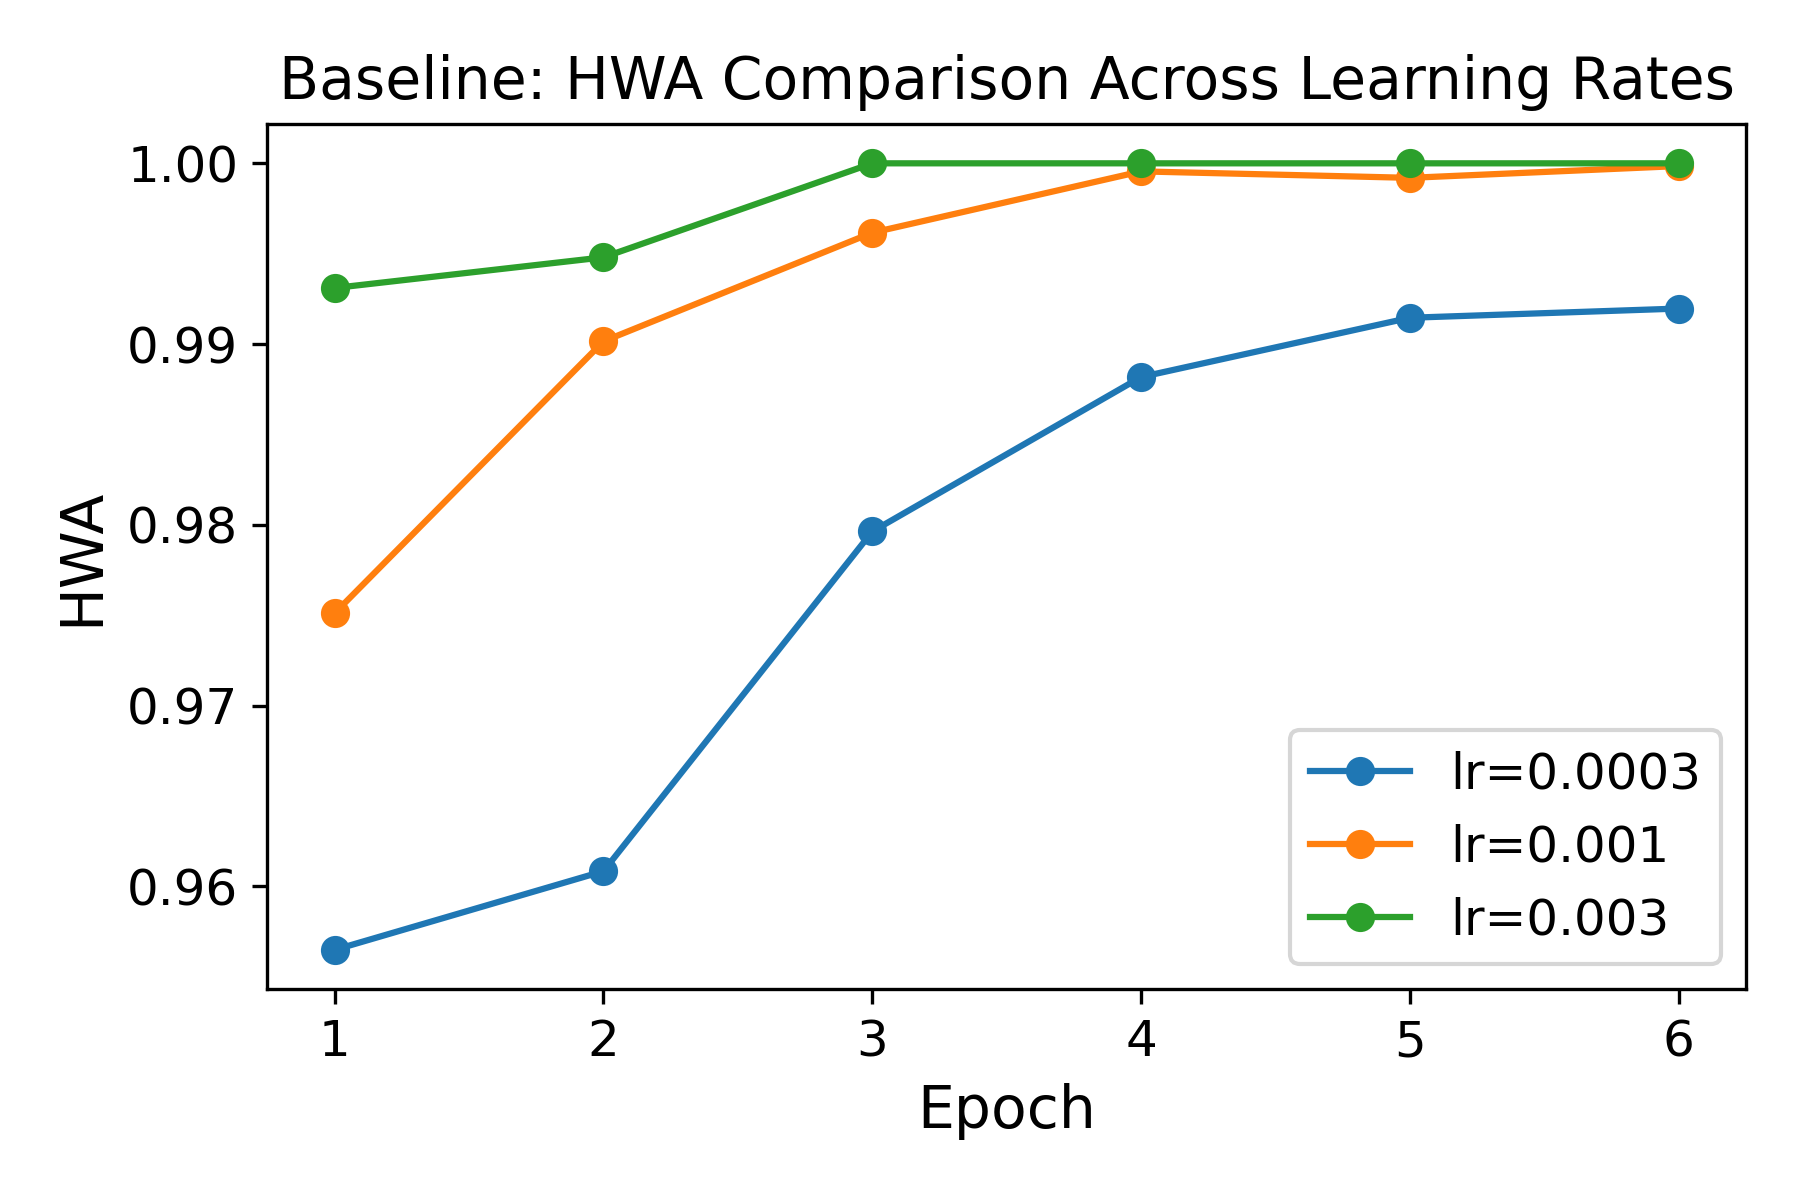
\includegraphics[width=\textwidth]{Baseline_HWA_Comparison.png}
    \caption{Training curves at various learning rates.}
\end{subfigure}
\hfill
\begin{subfigure}[b]{0.45\textwidth}
    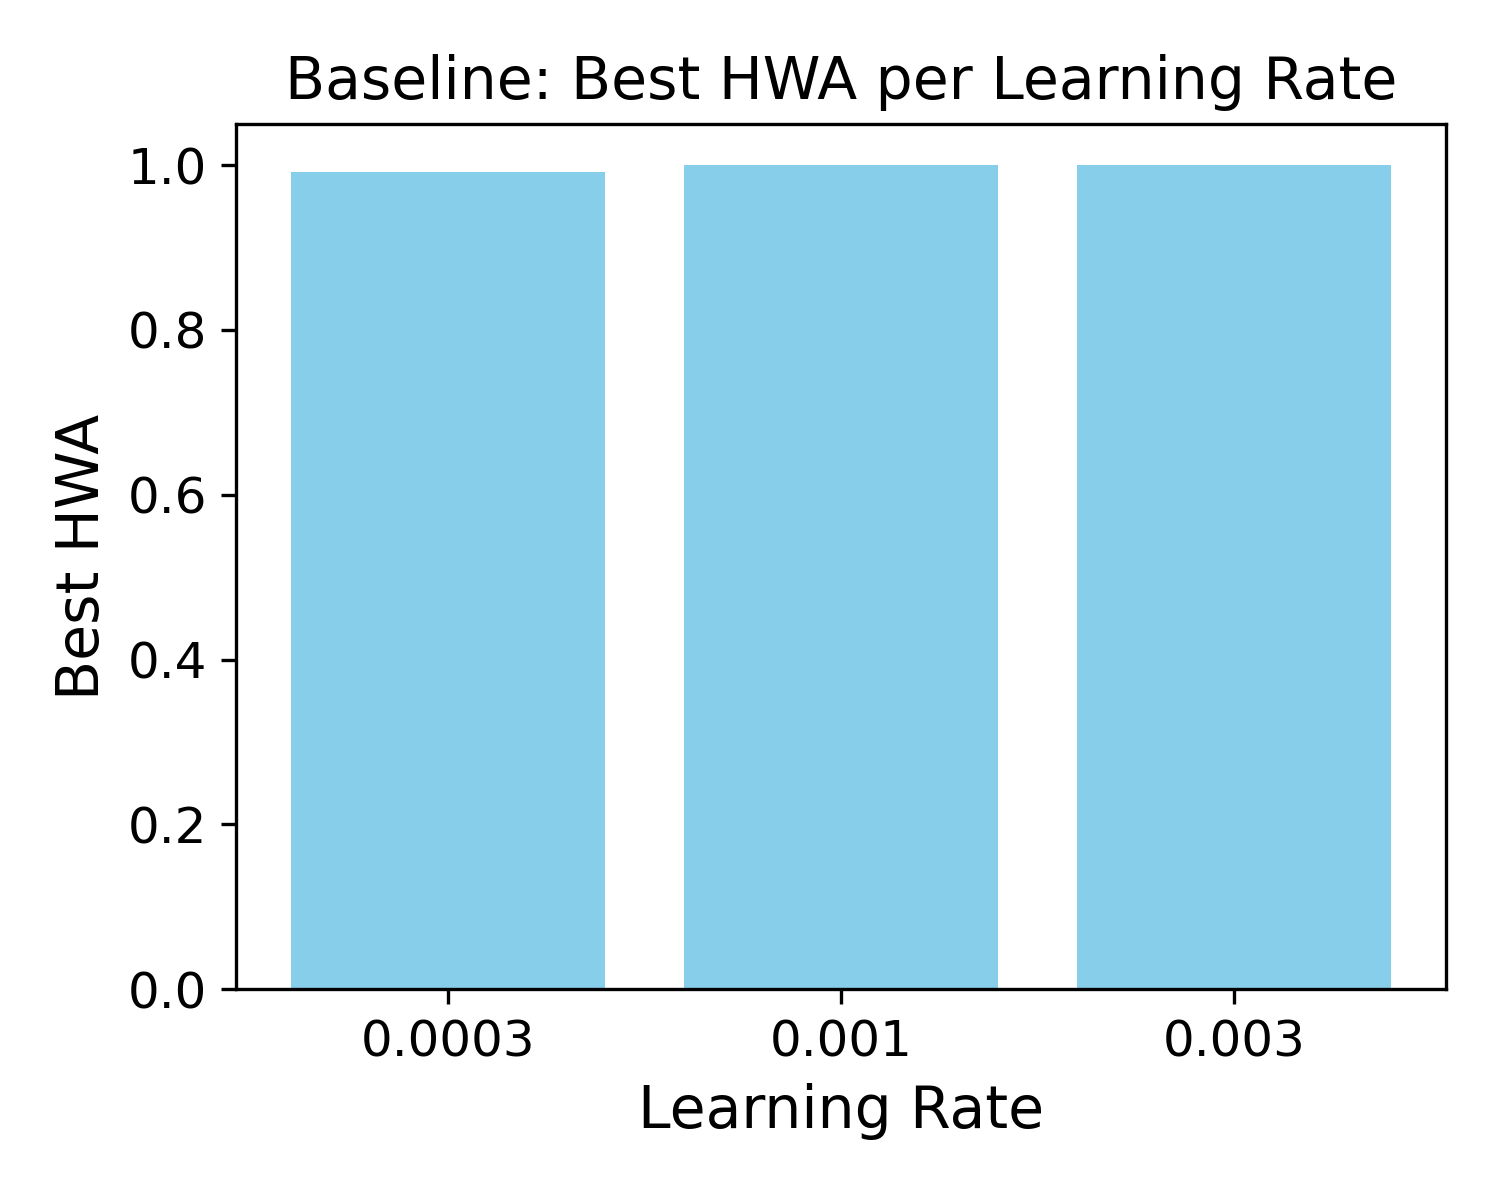
\includegraphics[width=\textwidth]{Baseline_Best_HWA.png}
    \caption{Near-perfect final accuracy post-training.}
\end{subfigure}
\caption{Models on \textit{SPR\_BENCH} with different settings converge equally fast and achieve uniformly high performance.}
\label{fig:baseline}
\end{figure}

\begin{figure}[t]
\centering
\begin{subfigure}[b]{0.45\textwidth}
    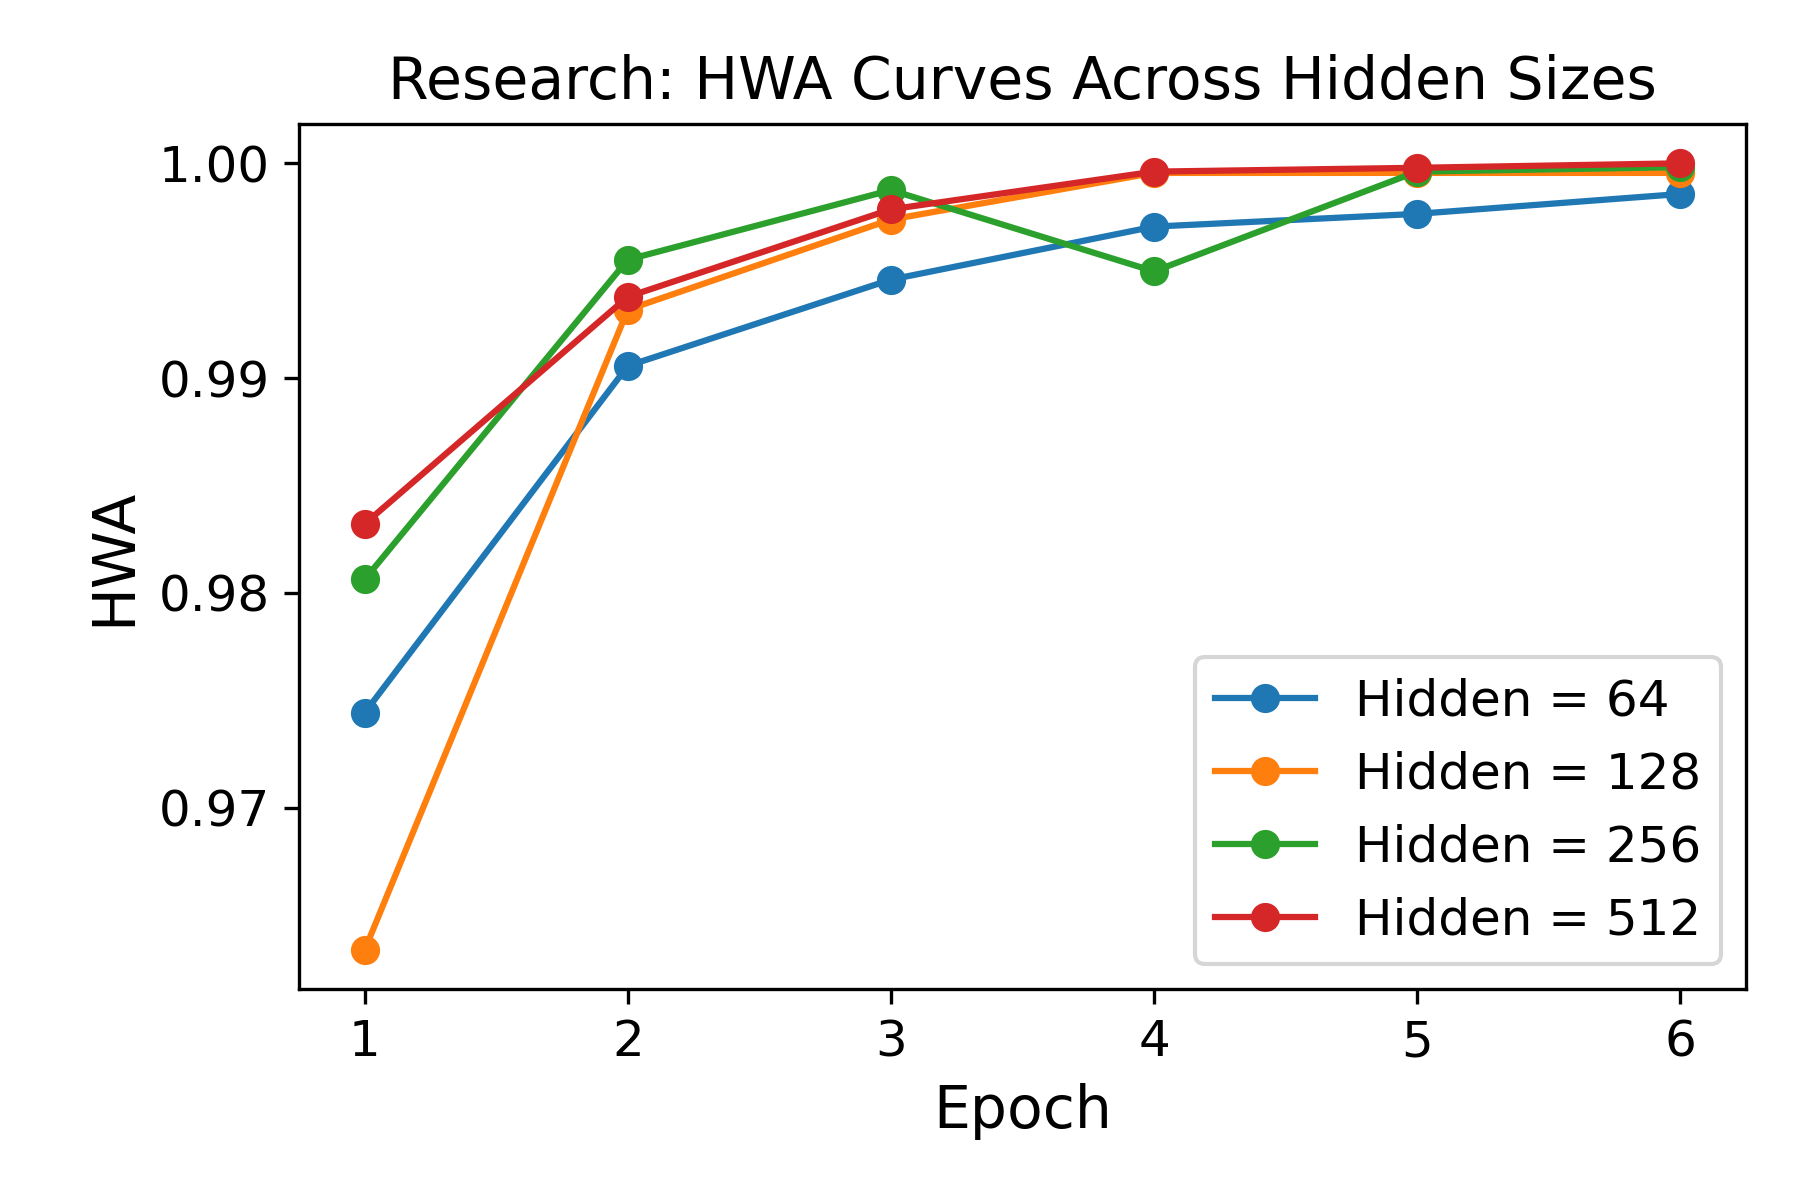
\includegraphics[width=\textwidth]{Research_HWA_Curves.png}
    \caption{Scaling hidden dimension from 64 to 512.}
\end{subfigure}
\hfill
\begin{subfigure}[b]{0.45\textwidth}
    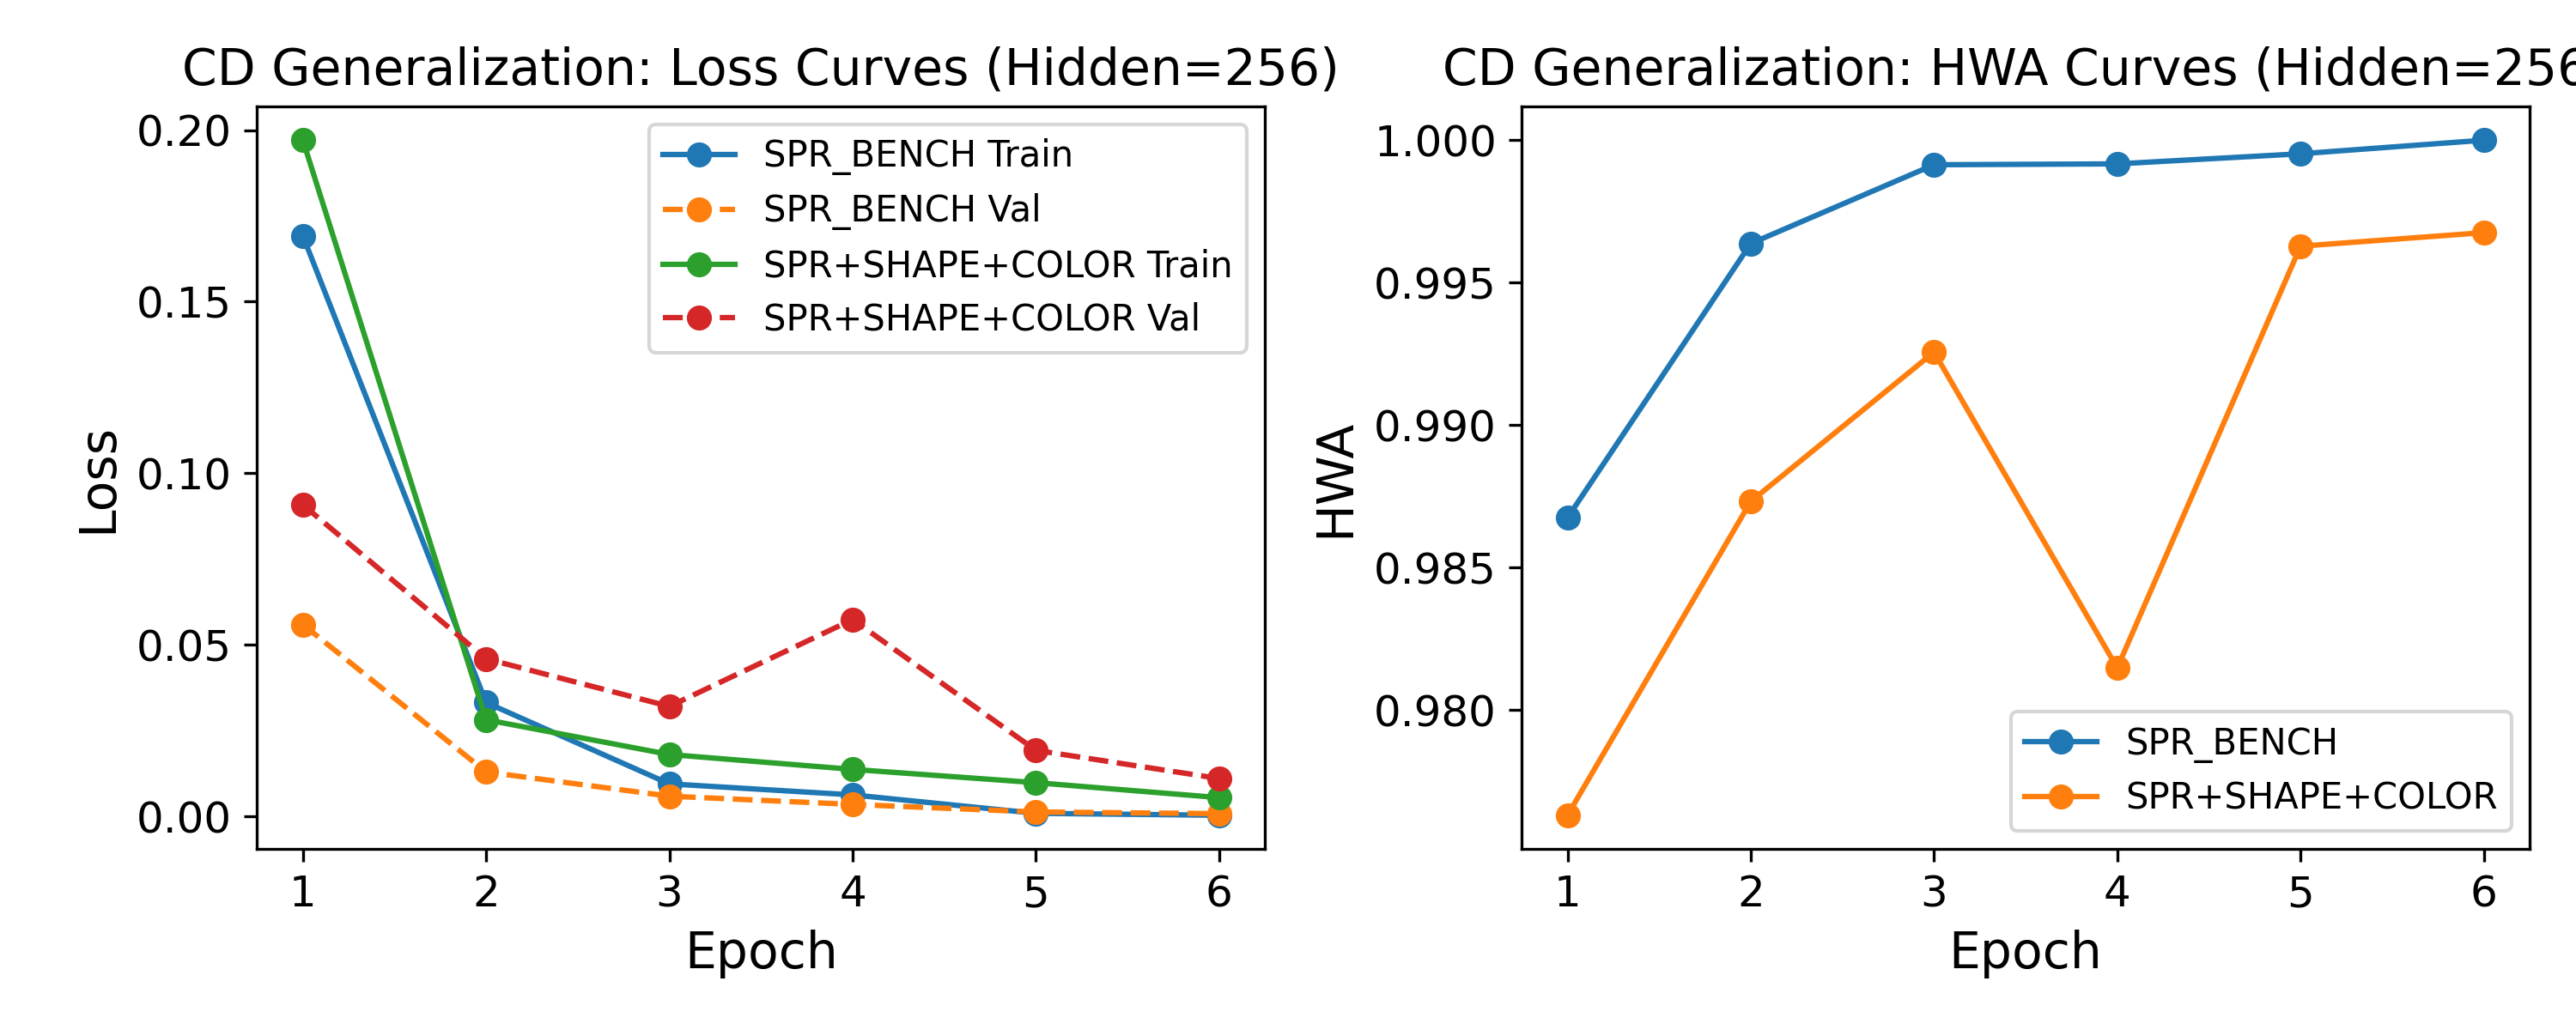
\includegraphics[width=\textwidth]{Abla_CD_Generalization_256.png}
    \caption{Cross-dataset generalization remains near 1.0 accuracy.}
\end{subfigure}
\caption{Even when increasing model capacity, performance does not degrade.}
\label{fig:research}
\end{figure}

\section{Conclusion}
Our investigation highlights that apparently difficult tasks can still yield trivial results, endangering robust evaluation. This work serves as a reminder to rigorously validate benchmark complexity. Future directions include curating datasets with realistic noise and variability, ensuring that cutting-edge methods are truly tested beyond simple convergence.

\bibliographystyle{iclr2024_conference}
\bibliography{references}

\clearpage
\appendix

\section{Supplementary Material}
Additional plots show similar convergence trends with alternate architectural changes. All results support our main claim: models easily overfit \textit{SPR\_BENCH} and fail to reveal meaningful performance differences.

\end{document}